\chapter{Проектирование и применение модульного технологического оборудования}\label{ch:ch2}

\section{Методика унификации модулей с электромагнитным креплением}

\subsection{Принципы унификации оборудования}

Проблема унификации оборудования стоит особняком в ряду проблем, возникающих в области стандартизации. На сегодняшний день унификация распространена повсеместно и включает в себя самые разные нормы, требования, процессы, методы и документы. Однако потребность в решении проблемы унификации по-прежнему существует. Данное утверждение подтверждается действующими нормативными документами. В данных нормативных документах регламентируются такие параметры, как номенклатура и содержание основных требований, предъявляемых к унификации, состав и структура проводимых работ по унификации и т.\,д. К сожалению, данные стандарты в первую очередь направлены на военно-промышленный комплекс, где вопросам стандартизации и унификации уделяется особое внимание. Поэтому на сегодняшний день можно постулировать, что проблемы общепромышелнной унификации и дальнейшее совершенствование теоретических основ унификации остаются крайне актуальными для нашей страны. 

Сейчас в промышленном производстве унификация практически забыта. Последнее обуславливается множеством факторов, к которым можно отнести несовершенное нормативно-правовое обеспечение и недостаточную научную проработанность унификации с точки зрения современного промышленного производства. Из значимых работ есть только учебные издания, которые описывают зачастую уже устаревшие нормы и правила. 

Безусловно, причиной недостаточно развития принципов унификации в нашей стране можно назвать отказ от плановой экономики и возникающих вследствие этого недочетов в управлении отдельными предприятиями, работающими по принципа рыночной экономики. Очевидно, что основная цель таких предприятий сиюминутная прибыль, при это решение более важных и перспективных в плане ценности конечного результата задач по большей части откладывается на неопределенный срок. 

Поэтому в настоящее время практически не появляются какие-либо индустриальные стандарты производства высокотехнологичной продукции. На первое место выходит защита собственных интеллектуальных интересов, а потенциальная выгода от работы в коллаборации с конкурентами представляется чем-то недостижимым. Конечно, решающую роль в формировании подобных отраслевых стандартов должно играть государство, но в рамках рыночной экономики открытым остается вопрос применимости стандартов <<навязанных>> сверху. Исходя из всего вышесказанного можно выделить следующие основные причины пренебрежения принципами унификации на современных предпритяиях:

\begin{itemize}
	\item отсутствие какой-то экономической заинтересованности во внедрении унифицированных составных частей в своих изделиях, если эти изделия разработаны другими предприятиями (хотя такие прецеденты существуют);
	\item отсутствие практики конкурсных разработок важных составных частей и изделий (за исключением работы в пользу государственных/оборонных предприятий);
	\item отсутствие четкой информация по унифицированным и стандартизованным составным частям распространенных изделий.
\end{itemize}

Учитывая вышесказанное, задача унификации модулей и шасси модульного технологического оборудования стоит достаточно остро. В то время как унификация немодульного оборудования важна в большей степени производителю, чтобы удешевить производство, обслуживание и ремонт, унификация модульного оборудования в значительной мере касается и потребителя. Унификация модулей и шасси позволят с одной стороны сократить их многообразие, а с другой увеличить количество возможных собираемых конфигураций. 

Основными инструментами унификации являются параметрические ряды и ограничения. Для составления параметрических рядов есть ряд правил, закрепленных в соответствующих нормативных документах.\footnote{ГОСТ 23945.0-80. Унификация изделий. Основные положения.}\footnote{РД 50-632-87 Методические указания. Унификация изделий построение параметрических и типоразмерных рядов деталей и сборочных единиц общемашиностроительного применения.} Обычно параметрические ряды составляются из некоторого ряда предпочтительных чисел,\footnote{ГОСТ 8032-84. Предпочтительные числа и ряды предпочтительных чисел.} представляющего собой числовую последовательность, полученную по определенному правилу, например, правилу арифметической или геометрической прогрессии.

\subsection{Особенности конструкции модулей}

Несомненно, модули могут различаться по размеру в зависимости от решаемой задачи. Причем, в соответствии с принципом унификации, система управления должна определять положение подключенного модуля самостоятельно и без необходимости ручной настройки или калибровки. Известно, что точность обработки зависит от точности взаимного геометрического положения всех компонентов промышленного оборудования. Этого чрезвычайно сложно достичь при применении модульного подхода, поскольку положение модуля относительно системы координат шасси заранее неизвестно.

Более высокую точность позиционирования можно получить, изменив способ установки модулей на подвеске каретки и, например, используя крепления <<ласточкин хвост>> с клиновым зажимом. Описанная схема широко применяется в быстросменных резцедержателях металлообрабатывающих станков. Такой подход обеспечивает отличную точность и повторяемость при переустановке модулей вручную. Однако это значительно усложняет общую конструкцию подвеса каретки из-за необходимости высокоточной обработки сопрягаемых деталей (требуется шлифование всех сопрягаемых поверхностей в соединении), а также увеличивается общий вес подвижной части в системе. Кроме того, все модули должны иметь одинаковые ответные части типа <<ласточкин хвост>>, размеры которых зависят не от размера самого модуля, а от размеров шасси. Следовательно, нарушается принцип универсальности, поскольку в этом случае невозможно установить малогабаритный модуль на большое шасси.

Усилия используемых в настоящее время магнитных крепления вполне достаточно для установки практически всех видов измерительных и обрабатывающих модулей. Однако, все эксперименты с обработкой металлов проводились на маломощных шпинделях при небольшой глубине резания. Последнее обусловлено небольшими габаритами и жесткостью экспериментальной установки. Однако, как уже отмечалось ранее, предполагается разработка линейки координатных платформ разного размера и жесткости. Очевидно, что для более габаритных платформ будут использоваться более тяжелые режимы обработки резанием, при которых возможен отрыв шпиндельного модуля от посадочной поверхности подвеса каретки. Данная проблема требует дополнительных исследований.

Наиболее целесообразным представляется использование электромагнитов вместо постоянных магнитов. Данное предположение подтверждается наличием на рынке специализированных сверлильных станков на магнитной подошве.\footnote{Электронный ресурс: {\tiny\url{https://www.bds-machines.com/magnetic-drilling-machines/mab-825-kts/}} (дата обращения: 20.09.2019).} С их помощью осуществляется сверление, рассверливание, зенкерование, нарезания резьбы даже фрезерование в различных металлоконструкциях в судостроении, тяжёлом машиностроении, при ремонте трубопроводов, при выполнении строительных работ и т. д. Широкое распространение подобных станков связано с применением современных электромагнитных плит с большой удерживающей силой, являющихся основанием станков. Данный положительный опыт может быть использован для модернизации предлагаемой концепции установки модулей.

Также стоит отметить, что одним из вариантов использования модульного оборудования является включение его в гибкие производственные линии, где потребуется автоматическая замена модуля с использованием промышленного робота-манипулятора. Анализ современного оборудования показал, что достаточное усилие прижатия клинового зажима может быть достигнуто только с помощью пневматических зажимов. Это приводит к необходимости дополнительной воздушной линии, что также усложняет первоначальный предложенный подход.

Вместо этого предлагается использовать магнитную систему крепления с дополнительной направляющей канавкой, расположенной в плоскости, параллельной направлению каретки~(рисунки~\cref{fig:quick-mount} и \cref{fig:quick-mount-1}). Описанная система крепления позволяет использовать модули любого размера; однако возникает проблема объединения систем координат модуля и основного шасси. В данной работе предлагается комбинированная система автоматического позиционирования модуля на подвеске каретки с использованием машинного зрения. Эта система определяет расположение специализированных оптических маркеров на шасси и автоматически изменяет геометрические параметры, используемые в системе управления.

\begin{figure}[ht]
	\centerfloat{
		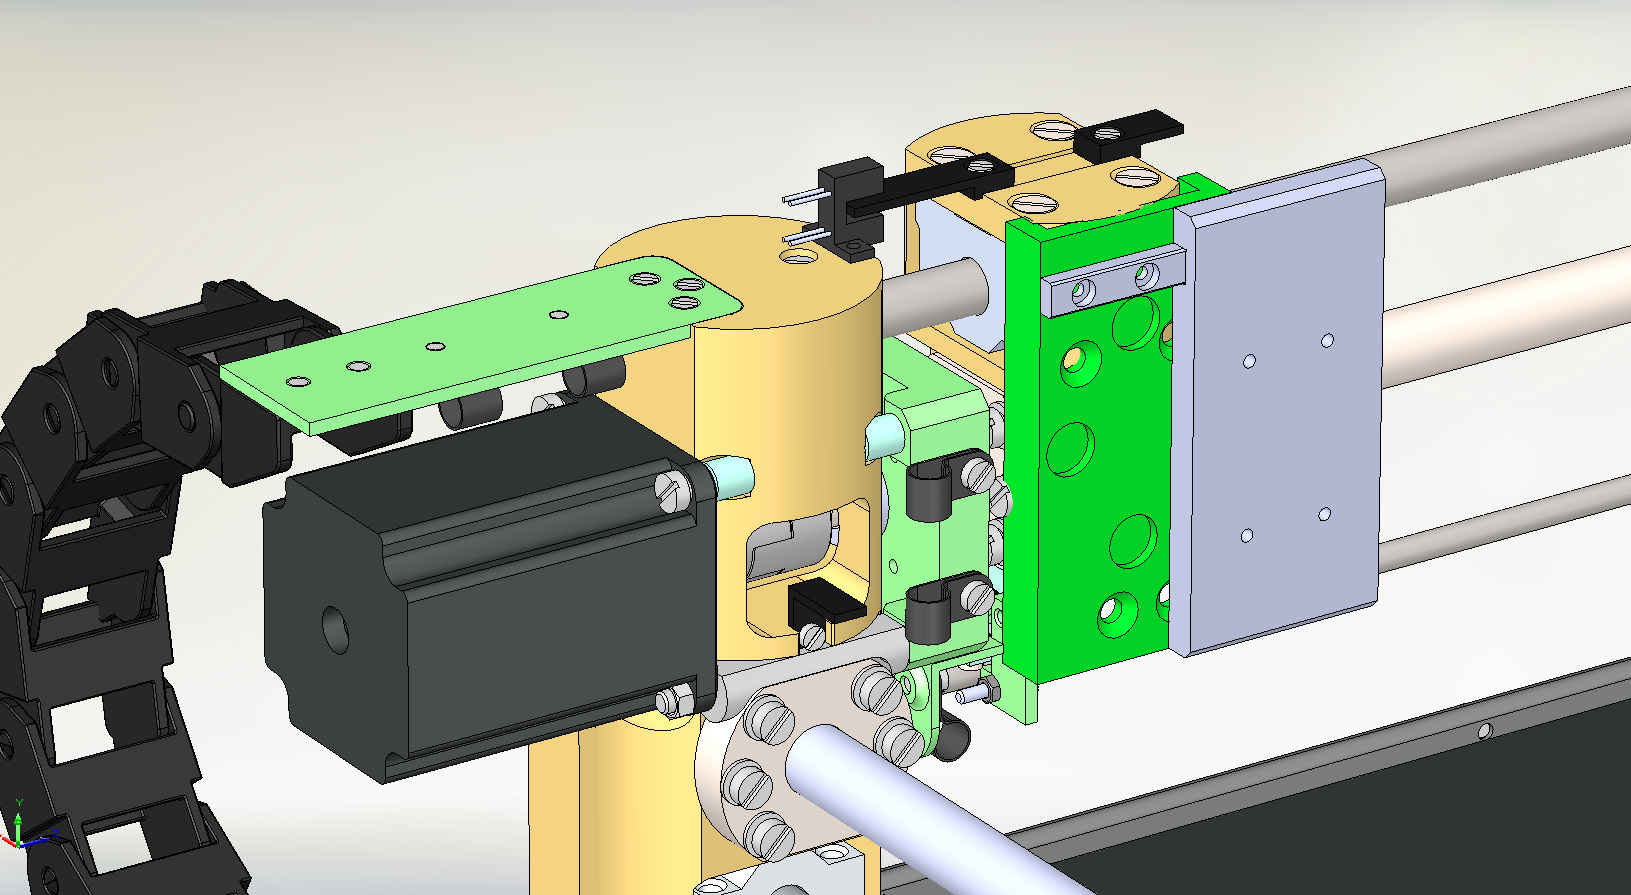
\includegraphics[width=0.7\textwidth]{ch-2/quick-mount}
	}
	\caption{Конструкция магнитного крепления модуля}\label{fig:quick-mount}
\end{figure}

\begin{figure}[ht]
	\centerfloat{
		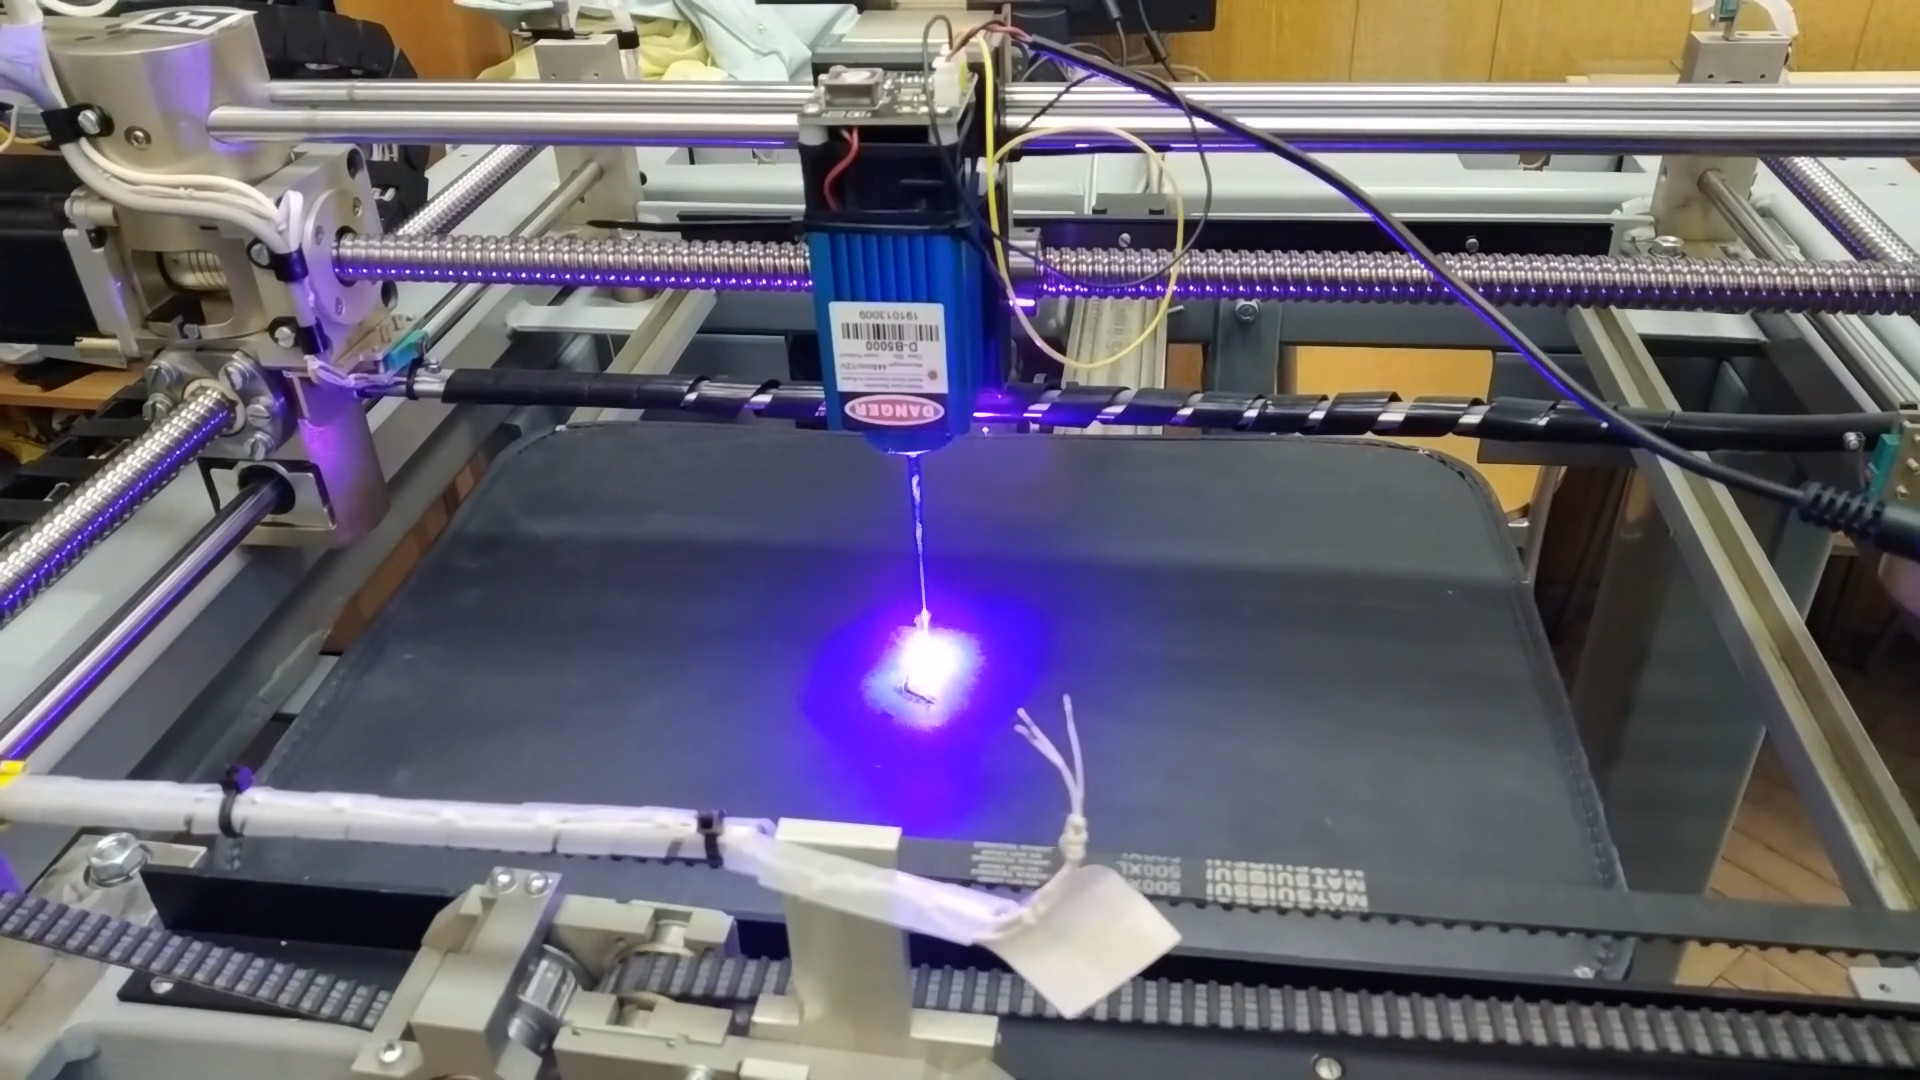
\includegraphics[width=0.7\textwidth]{ch-2/quick-mount-1}
	}
	\caption{Магнитного крепление с установленным лазерным модулем}\label{fig:quick-mount-1}
\end{figure}

\subsection{Этапы унификации модульного оборудования}

Первым этапом является определение параметров подлежащих унификации. Для модулей с электромагнитным креплением основными параметрами будут:

\begin{itemize}
	\item Грузоподъемность электромагнита.\footnote{сноска главный параметр}
	\item Ширина присоединительной поверхности модуля. 
	\item Глубина модуля.
	\item Ток потребления модуля.
\end{itemize}


Из данного списка необходимо выбрать главный параметр. Обычно главный параметр выбирают как параметр наиболее полно характеризующий несущую способность или другую эксплуатационную характеристику. Поскольку модули имеют различную функциональность, то в качестве главного параметра выбрана грузоподъемность электромагнита~\cref{eq-2-1}:

\begin{equation}
W = \{w_1, w_2, \ldots, w_n\}, n \in \mathbb{Z},
\label{eq-2-1}
\end{equation}

\noindent характеризующая выдерживаемое усилие. Этот параметр с одной стороны косвенно связан с массой модуля, а соответственно возможностью его установки на каретку того или иного шасси. С другой стороны он может быть связан с технологическими режимами работы модуля, например с силой резания при фрезеровании.

В качестве основных параметров выбраны~(рисунок~\cref{fig:geom-module}):

\begin{itemize}
	\item Ширина присоединительной поверхности модуля,\\$L = \{l_1, l_2, \ldots, l_n\}, n \in \mathbb{Z}$.
	\item Глубина модуля, $G = \{g_1, g_2, \ldots, g_n\}, n \in \mathbb{Z}$.
	\item Ширина модуля, $H = \{h_1, h_2, \ldots, h_n\}, n \in \mathbb{Z}$.
	\item Ток потребления модуля, $I = \{i_1, i_2, \ldots, i_n\}, n \in \mathbb{Z}$.
\end{itemize}

\begin{figure}[tbh]
	\centering
	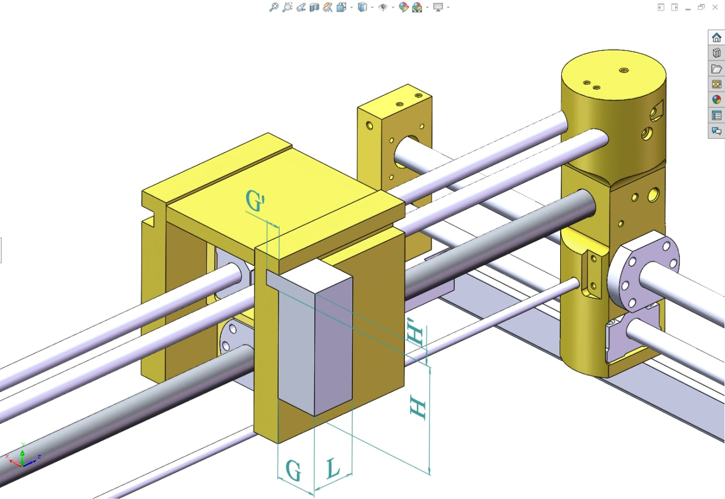
\includegraphics[width=\linewidth]{ch-2/geom-module}
	\caption{Параметры присоединительной поверхности модуля}
	\label{fig:geom-module}
\end{figure}

В качестве фиксированных параметров приняты:

\begin{itemize}
	\item Напряжение питания, $U$.
	\item Параметры ответной части паза, $G'$ и $H'$.
\end{itemize}

Напряжение питания выбрано в качестве фиксированного параметра, чтобы избежать применения преобразователей напряжения и использовать напряжение 24\:В де-факто ставшее промышленным стандартом. Параметры ответной части паза должны быть зафиксированы для обеспечения  широких возможностей по установки нескольких модулей одновременно. Следующим этапом необходимо определить ограничения выбранных параметров. Для модулей с электромагнитным креплением было выявлено пять ограничений.

\paragraph{Ограничение массы модуля в зависимости от грузоподъемности электромагнита.} При проектировании модуля необходимо учитывать его суммарную массу. Вес модуля должен быть меньше отрывного усилия в $\frac{1}{1-k}$ раз. Где $k$ "--- это коэффициент запаса. Формально ограничение может быть описано как:

\noindent $\rho : M \rightarrow P$ "--- соответствие <<модуль имеет массу>>.

\noindent $r : M \rightarrow W$ "--- соответствие <<электромагнит, установленный на модуль, имеет грузоподъемность>>.

\begin{equation}
m \in M: \rho(m) \leq r(m)
\end{equation}

\paragraph{Ограничение грузоподъемности электромагнита в зависимости грузоподъемности шасси.} При проектировании модуля необходимо учитывать что грузоподъемность электромагнита, а соответственно максимально устанавливаемая на шасси масса (масса модуля), должна была меньше грузоподъемности шасси c учетом коэффициента запаса~\cref{eq-2-2}.

\noindent $S = \{s_1, s_2, \ldots, s_n\}, n \in \mathbb{Z}$ "--- множество шасси.

\noindent $u: M \rightarrow S$ "--- соответствие <<модуль устанавливается  на шасси>>. 

\noindent $\vartheta: S \rightarrow P'$ "--- соответствие <<каретка шасси имеет грузоподъемность>> 

\begin{equation}
m \in M, s \in u(M): r(m) \leq \vartheta(s)
\label{eq-2-2}
\end{equation}

Если предполагается устанавливать данный модуль одновременно с другими, то~\cref{eq-2-3}:

\begin{equation}
m \in M, s \in u(M): \sum_{i=1}^{|M|}r(m_i) \leq \vartheta(s)
\label{eq-2-3}
\end{equation}

\paragraph{Ограничение тока потребления модуля в зависимости от максимального рабочего тока шасси.} Ток потребления модуля должен быть меньше рабочего тока шасси c учетом коэффициента запаса~\cref{eq-2-4}.

\noindent $M = \{m_1, m_2, \ldots, m_n\}, n \in \mathbb{Z} $ "--- множество модулей.

\noindent $i_{max} \in I$ "--- максимальный ток потребления.

\noindent $x: S \rightarrow i_{max}$ "--- <<соответствие шасси имеет максимальный рабочий ток>>.

\noindent $f: M \rightarrow I$ "--- соответствие <<модуль потребляет>>, тогда:

\begin{equation}
m \in M: f(m) \leq x(s)
\label{eq-2-4}
\end{equation}

Если предполагается устанавливать данный модуль одновременно с другими, то~\cref{eq-2-5}:

\begin{equation}
m \in M: \sum_{i=1}^{|M|}f(m_i) \leq x(s)
\label{eq-2-5}
\end{equation}

\paragraph{Ограничение глубины модуля в зависимости от рабочего пространства.} Глубина модуля определяет доступное рабочее пространство шасси в зависимости от общего рабочего поля шасси. С увеличением глубины модуля для обеспечение заданного рабочего пространства модуля необходимо увеличивать общее рабочее поля шасси. Тогда ограничение может быть записано как~\cref{eq-2-6}:

\noindent $S = \{s_1, s_2, \ldots, s_n\}, n \in \mathbb{Z} $ "--- множество шасси.

\noindent $G = \left \langle g_1, g_2, \ldots, g_n\right \rangle, n \in \mathbb{Z} $ "--- кортеж параметров глубины модулей.

\noindent $u: M \rightarrow S$ "--- <<соответствие модуль устанавливается на шасси>>.

\noindent $\delta: S \rightarrow B$ "--- соответствие <<шасси имеет размер рабочего пространства>>.

\noindent $y: M \rightarrow B'$ "--- соответствие <<для модуля задаётся минимальная размер рабочего пространства>>.

\noindent $\mu: M \rightarrow G$ "--- соответствие <<модуль имеет глубину>>.
 
\begin{equation}
m \in M, s \in u(M): \mu(m) + y(m) \leq \delta(s)
\label{eq-2-6}
\end{equation}

Если предполагается устанавливать данный модуль одновременно с другими, то~\cref{eq-2-7}:

\begin{equation}
m \in M, s \in u(M): max(\mu(M)) + y(m) \leq \delta(s)
\label{eq-2-7}
\end{equation}

\paragraph{Ограничение на ширину присоединительной поверхности модуля.} необходимо уместить $n$ модулей с шириной присоединительной поверхности $l_{m_i} \in L$ на каретке шасси шириной $l_\omega$ компактно. Сущность критерия компактности заключается в том, чтобы оставшееся свободное пространство оставалось полезным, где под полезностью понимается возможность установить хотя бы один модуль.

\noindent Для обеспечения вместимости достаточно: $\sum_{i=1}^{n}l_{m_i} \leq l_\omega$.
\noindent Тогда критерий компактности определяется как~\cref{eq-2-8}: 

\begin{equation}
\left ( l_\omega - \sum_{i=1}^{n} l_{m_i} \right )\rightarrow 0
\label{eq-2-8} 
\end{equation}

\noindent и имеет свой оптимум при~\cref{eq-2-9}:

\begin{equation}
\sum_{i=1}^{n} l_{m_i} = l_\omega.
\label{eq-2-9}
\end{equation}

\noindent Тогда~\cref{eq-2-10}:

\begin{equation}
L' \subset L, L'' \subset L: \sum_{i=1}^{|L'|}l_m + \sum_{i=1}^{|L''|}l_m = l_\omega
\label{eq-2-10}
\end{equation}

Этому условию удовлетворяют кратные ряды вида~\cref{eq-2-11}:

\begin{equation}
\left \{ \ldots, \frac{l_\omega}{n^2}, \frac{l_\omega}{n^1}, \frac{l_\omega}{n^0} \right \}, n \in \mathbb{Z}
\label{eq-2-11}
\end{equation}


Последним этапом необходимо сформировать параметрические ряды. Для параметра грузоподъемности электромагнита можно использовать ряд предпочтительных чисел, при этом ряд должен быть ограничен сверху грузоподъемностью шасси.

%--формула--

Параметрический ряд глубины модуля можно также сформировать из ряда предпочтительных чисел, при этом ряд должен быть ограничен сверху величиной равной разнице  рабочее поле шасси - минимальное желаемое рабочего поле модуля.

%--формула--

Параметр ширины присоединительной поверхности не может быть выбран из  ряда предпочтительных чисел, поскольку это не гарантирует обеспечения компактности. Тогда, исходя из критерия компактности можно синтезировать кратные ряды вида: 

%--формула--

Используя инструментарий полученных параметрических рядов, проектировщик модулей может добиться совместимости разрабатываемого модуля с шасси и модулями других разработчиков, при это не имея описания и документации на объекты совместимости. Кроме этого возможно достижение опережающей совместимости с объектами разработанными в будущем. Более того, появляется возможность на основе полученного формального описания рядов создать автоматизированную систему расчета параметров и проверки совместимости.

\section{Показатель целесообразности применения модульного оборудования}

Особенностью частных малых предприятий, занимающихся производством, является повышенная осторожность внедрения новых технологий и подходов. Зачастую это рассматривается как неоправданный, сложно поддающийся прогнозу риск, поскольку достаточно сложно произвести даже грубую предварительную оценку целесообразности применения того или иного новшества, а также определить готовность предприятия к внедрению. Обычно задача предварительной оценки внедрения новшества лежит исключительно в экономической плоскости. Рассчитываются такие показатели как индекс рентабельности (PI), срок окупаемости (PBP), внутренняя оценка доходности (IRR) и т.\:д. При этом величины параметров,на которые опираются показатели,  основываются на экспертных оценках. Все вышесказанное касается и внедрения новых видов технологического оборудования. Одним из самых распространенных способов общей оценки эффективности оборудования является показатель OEE~\cite{oee}.\footnote{Сокр. от англ. \textit{Overall Equipment Effectiveness} "--- общий эффективность оборудования.}

Общая эффективность оборудования (OEE) может быть точным представлением об общей производительности предприятия. Данная метрика стала развитием критерия Total Productive Maintenance (сокр. \textit{TPM}) и  Toyota Production System. OEE "--- это общее рассчитанное значение, которое представляет эффективность предприятия по трем ключевым показателям производительности:

\begin{itemize}
	\item Доступность оборудования, то есть возможность использования его в производственном процессе
	\item Производительность, то есть количество выпускаемой продукции в единицу времени без учёта брака.
	\item Приведённый уровень качества. 
\end{itemize}


Таким образом, расчёт OEE сводится к произведение показателей доступности, производства и качества, и его следует рассчитывать следующим образом:

\textit{Коэффициент доступности}. Это фактическое время выполнения технологических операций в течение определенного интервала времени, деленное на <<запланированное>> время выполнения для того же интервала. Например, работы, которые запланированы с учётом длительности рабочей смены, равной8 часам в день, 5 дней в неделю, имеет общую доступность 40 часов. Если фактическое время работы составляет 20 часов, результирующий коэффициент доступности составляет 50\,\%.

\textit{Производительность} "--- это фактическая валовая единица продукции, произведенная за определенный промежуток времени, деленная на количество единиц, которые должны были быть произведены. Технически, знаменатель в этом случае должен быть идеальным показателем, как определено технологической документацие, но в большинстве случаев возможно увеличение производительность по сравнению с первоначальной <<паспортной>> производительностью. Следовательно, для этого расчёта используется наилучшая достигнутая производительность. Например, когда запланировано производить 1000 единиц продукции в час, но при этом наилучшая продемонстрированная скорость составляет 2000 единиц в час, результирующая скорость производства составляет~50\,\%.

\textit{Показатель качества} является достаточно простым критерием. Это общее количество произведенных единиц продукции без брака, разделенное на общее количество произведенных единиц. Общее количество единиц продукции без брака определяется как общее количество произведенных единиц (брутто) за вычетом всего брака, как устранимого, так и неустранимого. Например, если производится всего 1000 единиц, но 100 единиц продукции отбраковываются, то числитель становится 900, а знаменатель "--- 1000, что даёт значение коэффициента равным~90\,\%.

Таким образом, после определения этих трех значений окончательный расчет OEE представляет собой просто произведение трёх значений, выраженных в процентах, то есть "--- это мультипликативный показатель который включает в себя три критерия~\cref{eq:oee}:\footnote{Электронный ресурс: \url{https://www.oee.com/} (дата обращения: 14.06.2019).}

\begin{equation}
OEE = A \times P \times Q,
\label{eq:oee}
\end{equation} 

\noindent где:

\noindent $A$ "--- критерий доступности (готовности) оборудования (англ. \textit{Availability});

\noindent $P$ "--- критерий производительности (англ. \textit{Performance});

\noindent $Q$ "--- критерий качества (англ. \textit{Quality})

Критерий доступности позволяет оценить простои оборудования, которые с одной стороны могут быть связаны с поломками, а с другой стороны "--- неравномерностью потока заказов. Для мелкосерийного и единичного дискретного производства, которые зачастую работают по принципу ETO\footnote{Сокр. от англ. \textit{Engineer-To-Order} "--- заказ на проектирование.} или MTO\footnote{Сокр. от англ. \textit{Made-To-Order} "--- заказ на изготовление.}, а не производят продукцию на склад, неравномерность потока заказов может привести к простою части оборудования.

Необходимо отметить особенности этих двух подходов к изготовлению продукции на заказа. MTO "--- производственный подход, при котором после получения подтвержденного заказа на продукты начинается полный производственный цикл их изготовления. Этот подход считается подходящим для продуктов с высокой степенью конфигурации, таких как автомобили, компьютерные серверы, или для продуктов, хранение запасов которых обходится дорого, например самолетов. MTO является основным подходом, используемый сегодня во многих отраслях. Он относится к изделиям, созданным до определения конечного покупателя, при этом объём производства определяется \textit{исторической информацией о спросе}.

Основными преимуществами подхода MTO в среде с большим разнообразием продуктов являются возможность предоставить заказчику точную требуемую спецификацию продукта, сокращение дорогостоящих товарных запасов, а также снижение риска устаревания запасов.
Основным недостатком MTO является то, что производители чувствительны к колебаниям рыночного спроса, что ведет к снижению загрузки производственных мощностей в производстве. Следовательно, для обеспечения эффективного использования производственных ресурсов подход MTO должен сочетаться с упреждающим управлением спросом, что является актуальной областью научных исследований.

С другой стороны, ETO "--- это производственный подход, обладающий следующими особенностями:

\begin{itemize}
	\item К срокам выполнения заказа следует добавить инженерные работы.
	\item После получения заказа от клиента технические требования и спецификации заказа в деталях не известны. Требуется значительный объем проектного и инженерного анализа.
\end{itemize}

ETO "--- это эффективный метод увеличения продаж и увеличения прибыльности для тех компаний, клиенты которых нуждаются в индивидуальных решениях, соответствующих их уникальным требованиям. Он начинается с продажи концепций продуктов, которые не имеют готового проекта и, как ожидается, позволят создать новый уникальный конечный продукт. Это может быть любой продукт, от корпоративных программных приложений до изделий машиностроения. Тем не менее, типичная среда ETO обычно имеет дело с проектированием и сборкой сложных машин и промышленного оборудования, спроектированных по индивидуальному заказу.

Возвращаясь к формуле расчёта показателя OEE~\cref{eq:oee-1}:

\begin{equation}
	A = \frac{OT}{PPT},
	\label{eq:oee-1}
\end{equation}

\noindent где:

\noindent $OT$ "---  время, когда оборудование действительно работало и выпускало продукцию.

\noindent $PPT$ "--- плановое время выпуска продукции.

Второй критерий, "--- критерий производительности, "--- позволяет внести в общий показатель составляющую, отвечающую за снижение производительности оборудования, сравнивая теоретический и практический выпуск продукции~\cref{eq:oee-1}.

\begin{equation}
	P = \frac{TP}{OT} \cdot \frac{1}{IRR},
	\label{eq:oee-2}
\end{equation}

\noindent где:
 
\noindent $TP$ "--- количество единиц продукции, выпущенное за операционное время OT,
\noindent $IRR$ "--- максимальное количество продукции, теоретически производимое в единицу времени.

И последний критерий, "--- критерий качества, "--- позволяет оценивать уровень брака выпускаемой продукции~\cref{eq:oee-1}.

\begin{equation}
	Q = \frac{GP}{TP}
	\label{eq:oee-3}
\end{equation}

\noindent где:

\noindent $GP$ "--- количество годной продукции, выпущенное за операционное время,
\noindent $TP$ "--- общее количество продукции, выпущенное за операционное время.

Учитывая вышесказанное, очевидно, что использовать такой показатель имеет смысл только после внедрения оборудования и оценки целесообразности применения его постфактум. Однако для текущей оценки эффективности работы оборудования данный показатель незаменим. Положительным считается результат величиной больше 0,75, а отрицательным меньше значения 0,65.\footnote{Электронный ресурст: \url{.promanage.com/7-blog/956-how-to-improve-oee/} (дата обращения 08.04.2020).} В случае неудовлетворительной оценки, где наибольший негативный эффект вносят составляющие критерия доступности и критерия производительности применение модульного оборудования позволяет привести к повышению значения OEE. Это связано с тем, что снижение производительности и доступности оборудования, вызывается образованием узких мест на производстве. При изготовлении деталей технологические операции имеют различную длительность. В случае, когда одна или несколько технологических операций при обработке партии деталей имеют большую по сравнению с остальными операциями продолжительность, оборудование начинает простаивать в ожидании предмета труда. В данных обстоятельствах модульное оборудование позволяет избавиться от узкого места меньшими затратами на дополнительное оборудование, за счет возможности временной реконфигурации других простаивающих единиц оборудования. 

Тем не менее, проведение анализа системы на наличие узких мест является трудоемким процессом, требующим временных затрат на сбор данных о функционировании системы. А в случае с новыми производственным предприятиями такую информации получить невозможно полностью из-за отсутствия полноценно функционирующего производства. При этом одним из этапов планирования нового производства является определение перечня необходимых ресурсов, куда включается технологическое оборудование. Для вышеуказанных целей предлагается использование \textit{показателя целесообразности модульности}. 

Для расчета показателя целесообразности модульности необходимо получить данные о номенклатуре производимых деталей. Для мелкосерийного и единичного производства эту информацию можно получить из имеющихся маршрутных карт групповых технологических процессов. Представим номенклатуру в виде множества~$N$~\cref{eq-2-15}:

\begin{equation}
N = \{D_1, D_2, \ldots, D_i\}, N = (D_i)_{i \in \mathbb{Z}},
\label{eq-2-15}
\end{equation}


где $D_i$ "--- это групповая деталь, представляющее собой множество классов технологических операций $p_m$ по классификатору технологических операций машиностроения и приборостроения~\cref{eq-2-16}:\footnote{Классификатор технологических операций машиностроения и приборостроения: 1 85 151. М.: Издательство стандартов, 1987.}

\begin{equation}
D = \{p_1, p_2, \ldots, p_m\},
\label{eq-2-16}
\end{equation}

\noindent В соответствие каждой групповой детали ставится планируемый объем выпуска~\cref{eq-2-17}:

\begin{equation}
f: D \rightarrow v_i, V \in \mathbb{Z}
\label{eq-2-17}
\end{equation}

На следующем этапе необходимо найти групповые детали с максимальным объемом выпуска (это может быть одна деталь или несколько). Данную процедуру представим в виде композиции функций~\cref{eq-2-18}:

\begin{equation}
\begin{split}
f &\circ g, \\
g: V \rightarrow N'': \forall v = V_max f(D), v \in V, \\
\end{split}
\label{eq-2-18}
\end{equation}

%\begin{equation}
%f \circ g,
%\end{equation}
%
%\begin{equation}
%g: V \rightarrow N'': \forall v = V_max f(D), v \in V,
%\end{equation}

\noindent где $V$ "--- кортеж, содержащий значения объемов выпуска для каждого вида изделий. Тогда $G=({N''}_i)_{i \in J}$ -- это семейство групповых деталей с максимальным объемом выпуска.
%ЧТО ТАКОЕ J?
Отсюда коэффициент целесообразности будет можно выразить следующим образом~\cref{eq-2-19}:

\begin{equation}
\epsilon = \frac{\big|\bigcup G \big|}{\big|\bigcup N \big|}
\label{eq-2-19}
\end{equation}

\noindent при $\epsilon \rightarrow 1$, модульность нецелесообразна.

\noindent при $\epsilon \rightarrow 0$, модульность целесообразна.

\paragraph{Описание маршрутного технологического процесса изделия <<Гироподвес>>.}

В качестве пример был рассмотрен технологический процесс изготовления изделия <<Гироподвес>>. Выбор был обусловлен тем фактом, что вся конструкторская документация на данное изделие находится в свободном доступе и может быть использована для создания и оптимизации маршрутной технологии для модульного технологического оборудования. Расчетные параметры технологических операций данного технологического процесса будут использоваться в оставшихся разделах данной главы.

Изделие <<Гироподвес>>~(рисунок~\cref{fig:gimbal}) представляет собой подвижную платформу, на которой может быть закреплена камера. Задача данного изделия "--- стабилизировать положение камеры по осям крена, тангажа и рысканья. Изделие состоит из следующих узлов:

\begin{itemize}
	\item Пластиковые корпусные детали, которые могут быть распечатаны на установке послойного наплавлени (трёхмерном принтере)~(рисунок~\cref{fig:gimbal-1}).\footnote{Электронный ресурс: \url{https://www.thingiverse.com/thing:1247236} (дата обращения: 16.03.2020).} 
	\item Печатная плата~(рисунок~\cref{fig:gimbal-2}).\footnote{Электронный ресурс: \url{https://github.com/olliw42/storm32bgc} (дата обращения: 26.07.2020).}
	\item Стандартные и покупные изделия.
\end{itemize}

\begin{figure}[htb]
	\centerfloat{
		\hfill
		\subcaptionbox{\label{fig:gimbal-1}}{%
			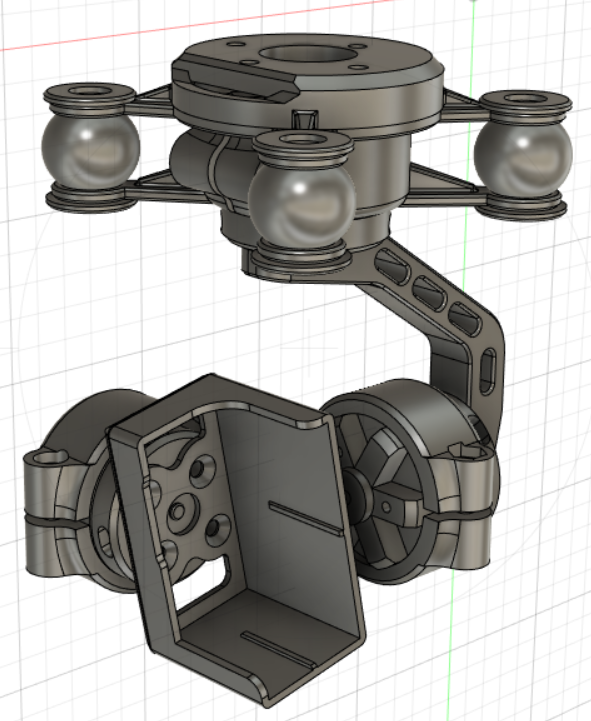
\includegraphics[width=0.33\linewidth]{ch-2/gimbal-3d}}
		\hfill
		\subcaptionbox{\label{fig:gimbal-2}}{%
			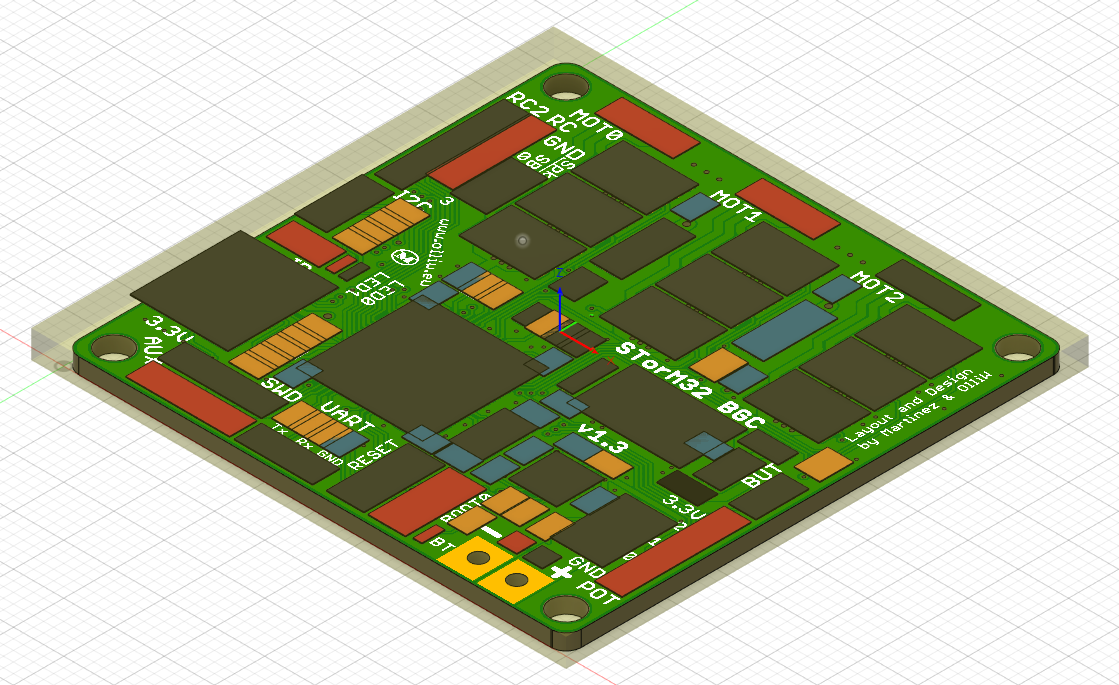
\includegraphics[width=0.33\linewidth]{ch-2/gimbal-pcb}}
		\hfill
		\subcaptionbox{\label{fig:gimbal-3}}{%
			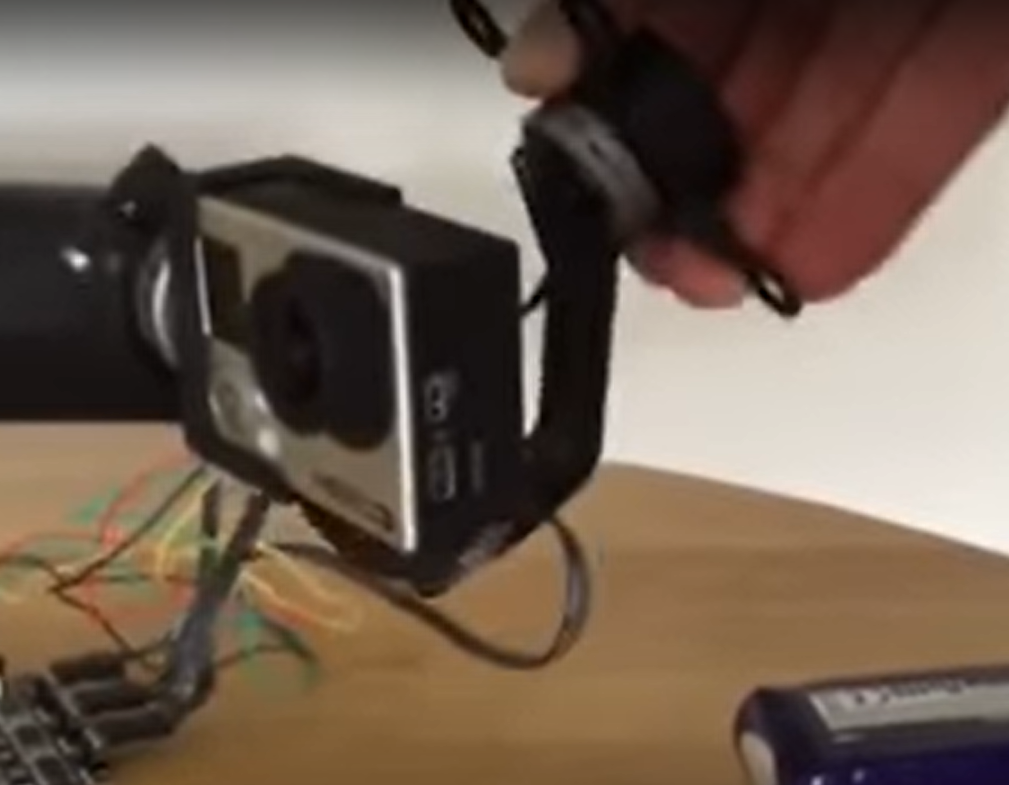
\includegraphics[width=0.33\linewidth]{ch-2/gimbal}}
		\hfill
	}
	\caption[Изделие <<Гироподвес>>]%
	{Изделие <<Гироподвес>>: трёхмерная модель (\textit{а}), печатная плата  (\textit{б}), готовое изделие (\textit{в}).}\label{fig:gimbal}
\end{figure}

Последовательность операций изготовления корпусных деталей на установке послойного направления представлена в таблице~\cref{tab:case}, последовательность изготовления печатной платы представлена в таблице~\cref{tab:pcb}.\footnote{Маршрутная карта представлена в приложении~\cref{app:A}.}

\begin{table} [!htb]
	\centering
	\caption{Последовательность операций изготовления корпусных деталей изделия <<Гироподвес>>} \vspace{4pt}
	\label{tab:case}
	\begin{threeparttable}
		\begin{tabularx}{\linewidth}{ll}
			\toprule
			\textbf{Код операции\tnote{1}} & \textbf{Наименование операции} \\
			\midrule
			6051 & Экструзия заготовок \\
			0108 & Слесарная \\ 
			4232 & Сверлильная с ЧПУ \\
			\bottomrule
		\end{tabularx}
		\begin{tablenotes} \footnotesize
			\item [1] Код из классификатора операций 1 85 151.
		\end{tablenotes}
	\end{threeparttable}
\end{table}

\begin{table} [!htb]
	\centering
	\caption{Последовательность операций изготовления печатной платы изделия <<Гироподвес>>} \vspace{4pt}
	\label{tab:pcb}
	\begin{threeparttable}
		\begin{tabularx}{\linewidth}{ll}
			\toprule
			\textbf{Код операции\tnote{1}} & \textbf{Наименование операции} \\
			\midrule
			4232 & Сверлильная с ЧПУ \\
			0109 & Зачистка \\
			0191 & Обезжиривание химическое \\
			6077 & Ламинирование пленочного фоторезиста \\
			5541 & Экспонирование \\
			5545 & Проявление \\
			0151 & Травление химическое \\
			0195 & Удаление покрытий \\
			6077 & Ламинирование паяльной маски \\
			5541 & Экспонирование \\
			5545 & Проявление \\
			0127 & Промывка растворителями \\
			6077 & Ламинирование трафаретных чернил \\
			5541 & Экспонирование \\
			5545 & Проявление \\
			0127 & Промывка растворителями \\
			4234 & Фрезерная с ЧПУ \\
			0158 & Дозирование по объему \\
			8878 & Монтаж комплектующих изделий \\ 
			8035 & Пайка готовым припоем в нейтральной газовой среде в печи \\
			\bottomrule
		\end{tabularx}
		\begin{tablenotes} \footnotesize
			\item [1] Код из классификатора операций 1 85 151.
		\end{tablenotes}
	\end{threeparttable}
\end{table}



\paragraph{Пример расчета коэффициента целесообразности.}

На производстве имеется 3 маршрутные карты групповых технологических процессов:

\begin{itemize}
	\item Маршрутная карта изготовления пластикового корпуса методом послойного наплавления, объём выпуска 100 единиц в год ($D_{case}$).
	\item Маршрутная карта изготовления печатной платы, объём выпуска 300 единиц в год ($D_{pcb}$).
	\item Маршрутная карта изготовления печатной платы с поверхностным монтажом электронных SMD-компонентов, объём выпуска 200 единицы в год~($D_{smd}$).
\end{itemize}

Здесь и далее четырёхзначные числа в скобках означают коды операций в классификаторе операций~\cref{eq-2-20}.

\begin{equation}
\begin{split}
	N &= \{D_{case}, D_{cb}, D_{smd}\} \\
	D_{case} &= \{005, 010\} \\
	D_{pcb} &= \{010, 015\} \\
	D_{smd} &= \{010, 015, 020, 025\}
\end{split}
\label{eq-2-20}
\end{equation}

\noindent Тогда~\cref{eq-2-21}:

\begin{equation}
\begin{split}
G &= (\{010, 015\}) \\
\bigcup G &= (\{010, 010\}) \\
\bigcup N &= \{005, 010, 015, 020, 025\} \\
\epsilon &= \frac{\big|\bigcup G \big|}{\big|\bigcup N \big|} = \frac{2}{5} = 0,25
\end{split}
\label{eq-2-21}
\end{equation}

Для проверки достоверности результата был проведен вычислительный эксперимент в системе Anylogic. Групповой технологический процесс изготовления печатной платы был представлен в виде диаграммы процесса с помощью дискретно-событийного метода.\footnote{Электронный ресурс: \url{https://www.anylogic.ru/use-of-simulation/discrete-event-simulation/} (дата обращения: 13.12.2018)} При этом было построено две диаграммы: для процесса использующего модульное оборудование~(рисунок~\cref{fig:oee-module}) и использующего немодульное оборудование (ссылка картинка).

\begin{figure}[!p]
	\centerfloat{
		\hfill
		\subcaptionbox{\label{fig:oee-module-1}}{%
			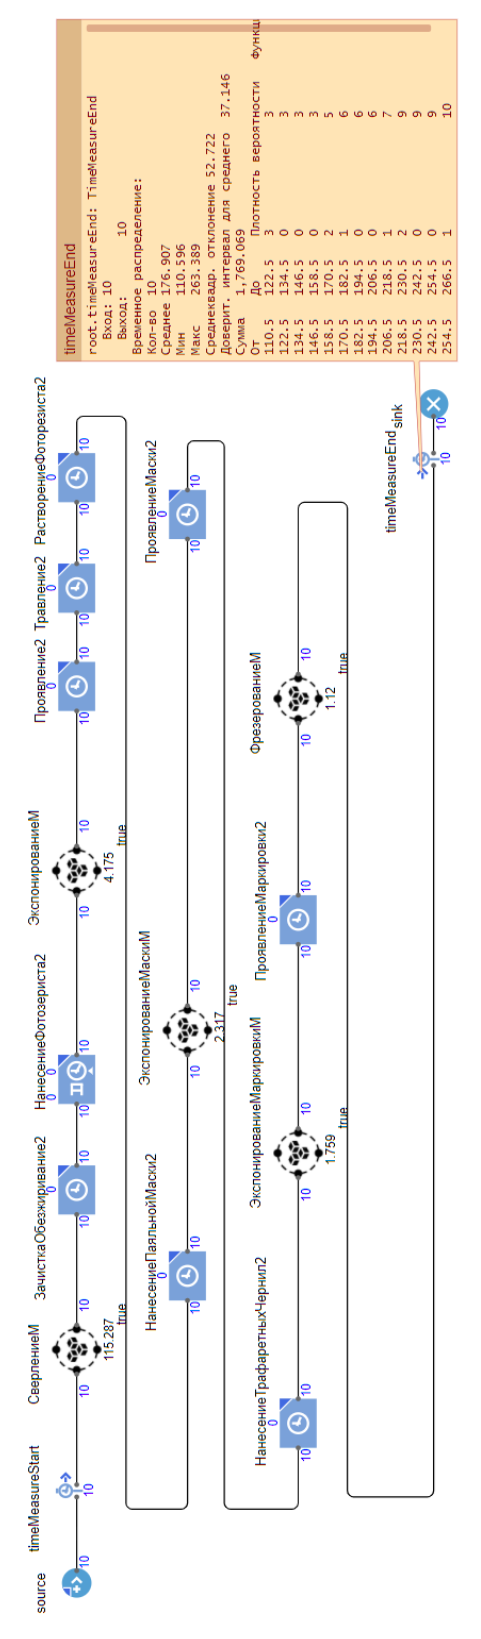
\includegraphics[width=0.42\linewidth]{ch-2/oee-module}}
		\hfill
		\subcaptionbox{\label{fig:oee-module-2}}{%
			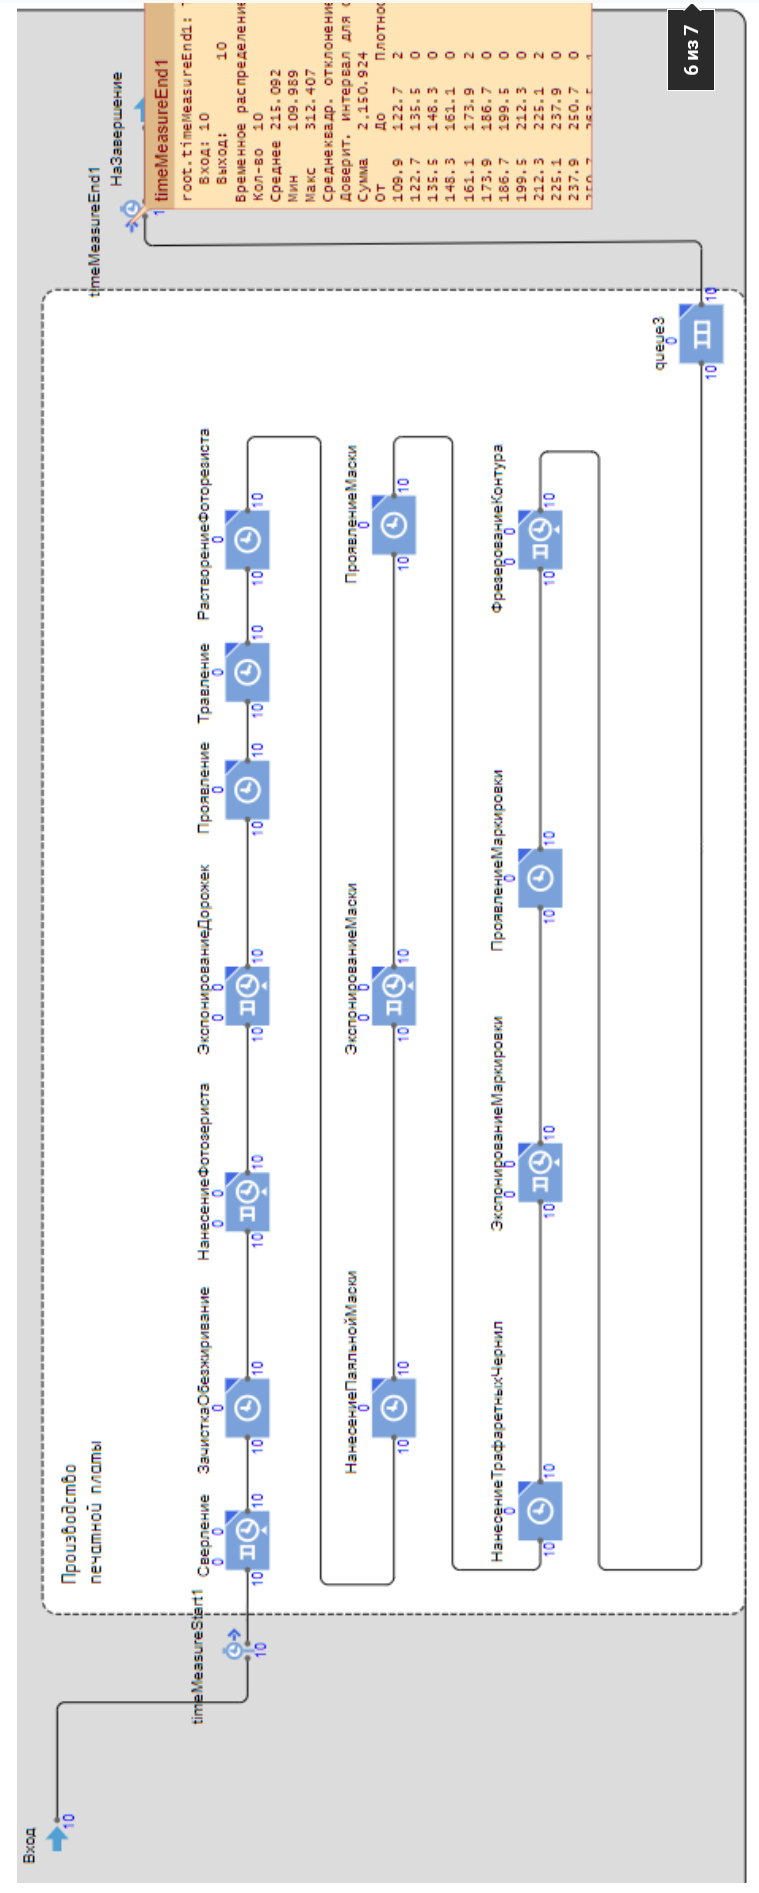
\includegraphics[width=0.52\linewidth]{ch-2/oee-no-module}}
		\hfill
	}
	\caption[Диаграмма процесса производства печатной платы для модульного и немодульного оборудования]%
	{Диаграмма процесса производства печатной платы для модульного (\textit{а}) и немодульного (\textit{б}) оборудования}\label{fig:oee-module}
\end{figure}

В процессе симуляции было обнаружено узкое место процесса на операции <<сверление>>, поскольку длительность её выполнения превосходила все остальные операции. Для повышения производительности, а соответственно снижения времени технологического цикла было предложено увеличить количество сверлильного оборудования. При этом для немодульного оборудования необходимо было добавить два дополнительных сверлильных станка, в то время как для модульного подхода было добавлено два сверлильных модуля, а шасси были переконфигурированы с простаивающих установок печати, монтажа и дозирования. В результате был получен прирост производительности в~\SI{18}{\percent}. Результаты вычислительного эксперимента представлены в таблице~\cref{tab:mod-nomod}.

\begin{table} [!htb]
	\centering
	\caption{Длительность технологического цикла производства партии печатных плат объёмом 10 единиц} \vspace{4pt}
	\label{tab:mod-nomod}
	\begin{threeparttable}
		\begin{tabularx}{\linewidth}{llr}
			\toprule
			\textbf{Тип оборудования} & \textbf{Перечень оборудования}    & \textbf{Время, мин.} \\
			\midrule
			Модульное                 & \begin{tabular}{@{}l@{}}
											3 сверлильных станка\\ 
											1 установка экспонирования\\
											1 фрезерный станок
										\end{tabular}                     & 29,5 \\
			Немодульное               & \begin{tabular}{@{}l@{}}
											1 модуль экспонирования\\       
											1 модуль фрезерования\\
											3 модуль сверления\\
											6 шасси\tnote{1}
										\end{tabular}                     & 36 \\	
			\bottomrule
		\end{tabularx}
		\begin{tablenotes} \footnotesize
			\item [1] Три единицы шасси снимаются с простаивающих установок печати, монтажа и дозирования.
		\end{tablenotes}
	\end{threeparttable}
\end{table}


\section{Оптимизация парка модульного технологического оборудования}
	 
\subsection{Определение требований к комплект модульного технологического оборудования и задачи оптимизации}

Комплектом технологического оборудования называется часть парка оборудования предприяния, используемого для реализации конкретного технологического процесса. Под парком технологического оборудования принимается совокупность оборудования, выполняющего технологические операции в автоматизированном режиме на одном предприятии. Парк технологического оборудования -- это важный производственный ресурс, определяющий такие характеристики производственного процесса как производительность, стоимость и качество выходной продукции. При этом производительность определяется с одной стороны производительностью каждой единицы оборудования по отдельности, а с другой, количеством единиц оборудования, работа которых может осуществляться параллельно.  Вместе с этим, оборудование -- это один из самых дорогостоящих ресурсов, требующий значительных затрат как на начальном этапе организации производства, так и в процессе эксплуатации. На данный момент наиболее дорогостоящим остается технологическое оборудование с ЧПУ. Это связано с рядом причин:

\begin{itemize}
	\item Высокая стоимость приводов движущей части технологического оборудования, особенно в случае применения сервоприводов.
	\item Сложность реализации системы управления, алгоритмы которой зачастую засекречены производителями.
	%* -- что-то еще? --
\end{itemize}

При организации парка оборудования важно, чтобы он отвечал следующим требованиям:

\begin{itemize}
	\item Обеспечение достаточного уровня автоматизации, соответствующего современным достижениям в науке и технике, в том числе использование ЧПУ.
	\item Обеспечение постепенного обновления имеющегося парка технологического оборудование.
	\item Применение производительных способов обработки.
	\item Гибкость парка оборудования при смене объемов и номенклатуры производства.
	\item Высокая отказоустойчивость.
\end{itemize}

Формирование парка оборудования это комплекс мероприятий, требующий точно определить и обосновать величину потребности в технологическом оборудовании, поскольку как недостаток, так и излишнее количество оборудования оказывают негативный эффект. Недостаточное количество технологического оборудования  приводит к ряду негативных эффектов:

\begin{itemize}
	\item Образованию узких мест.
	\item Повышенной загруженности определенных единиц оборудования.
	\item Простою определенных единиц оборудования в ожидании предмета труда для обработки.
	\item Межоперационное пролеживание предметов труда.
	\item Низкая отказоустойчивость.
\end{itemize}


Наряду с этим, излишнее количество также влечет к образованию простоев из-за малой загрузки и дополнительным финансовым издержкам. 

Учитывая вышесказанное, становится очевидной необходимость решения задачи оптимизации комплекта технологического оборудования, которая заключается в  определение оптимального количества необходимых единиц оборудования.

Комплект модульного технологического оборудования может как формировать комплект технологического оборудования полностью, так и только его часть. Предлагаемое модульное технологическое оборудование строится на основе базового агрегата, "--- координатного шасси, "--- отвечающего за перемещение каретки и установленных на неё модулей. Управление происходит также как и у немодульного оборудования с ЧПУ с помощью G-код программ и коротких команд. Применение электромагнитного крепления модулей и программного обеспечения с автоматической инициализацией и установкой связью с шасси позволяет не тратить большое количество времени на реконфигурацию машин. Отсюда наблюдается тенденция такого оборудования:

\begin{itemize}
	\item К повышению гибкости комплекта оборудования за счет возможной быстрой реконфигурации единиц модульного технологического оборудования.
	\item К повышению отказоустойчивости за счет возможной быстрой реконфигурации простаивающего оборудования.
	\item К повышению производительности меньшим эквивалентным количеством модульного оборудования, чем немодульного оборудования.
\end{itemize}

Тогда в случае с модульным технологическим оборудованием задача оптимизации преобразуется в задачу определения оптимального количества шасси и модулей для одного или нескольких технологических процессов.

\subsection{Целевая функция оптимизации комплекта модульного технологического оборудования}

Оптимизация "--- это выбор наилучшего варианта из возможных на основе одного или нескольких критериев. Для оптимизации комплекта модульного технологического оборудования необходимо рассматривать два критерия "--- стоимость предлагаемого комплекта оборудования и длительность технологического цикла. Фактически задача оптимизации сводится к задаче двухкритериальной оптимизации, где оба вышеуказанных критерия должны подвергаться минимизации.

Решение задач многокритериальной оптимизации является достаточно сложным и ресурсоёмким, поэтому по-возможности сводится к переходу от многокритериальной задачи к однокритериальной. Такой переход осуществляется за счет свертки. Самым распространенным способом свертки является аддитивная свертка\footnote{Васильев В.\,П., Мельник А.\,О. Решение многокритериальных задач принятия решения посредством смешанной свертки критериев //Современные инновационные технологии и проблемы устойчивого развития общества. "--- 2018. "--- С. 163-168.}, основанная на принципе взаимных компенсаций. Однако для обеспечения корректной компенсации критерии с разными единицами измерения следует нормировать.
 
Предлагается целевая функция оптимизации модульного технологического оборудования следующего вида~\cref{eq-2-22}:

\begin{equation}
f(t, c, \{m_1, m_2, \ldots m_n \}) = k_t \cdot \frac{t}{t_{norm}} + k_c \cdot \frac{c}{c_{norm}} + \sum_{i=0}^{n}k_i \cdot m_i, n \in \mathbb{Z},
\label{eq-2-22}
\end{equation}

\noindent где:
\noindent $k_t$, $k_c$, $k_i$ "--- весовые коэффициенты,
\noindent $t$ "--- время технологического цикла,
\noindent $t_{norm}$ "--- нормирующий множитель времени технологического цикла,
\noindent $с$ "--- количество шасси,
\noindent $c_{norm}$ "--- нормирующий множитель количества шасси,
\noindent $m_i$ "--- количество модулей определенного типа,\footnote{Модули относятся к одному типу, если выполняют операции одного класса.} выполняющих операцию определенного класса.

В качестве нормирующего множителя $t_{norm}$ используется длительность технологического цикла, рассчитанного для случая, где количество шасси соответствует количеству типов модулей, а количество модулей каждого типа принято за единицу. В качестве нормирующего множителя $c_{norm}$ используется количество шасси равное количеству типов модулей.

\subsection{Расчёт весовых коэффициентов}

Весовые коэффициенты необходимы для того, чтобы указать степень важности того или иного критерия в свертке. Зачастую для получения значений весовых коэффициентов прибегают к экспертной оценки, с использованием различных методов: метода анализа иерархий, метода парного сравнения, метода ранжирования, метода приписывания баллов и т.\,д. Основная сущность этих методов сводятся к переводу качественной оценки эксперта или группы экспертов в некоторое числовое значение.  Однако весовые коэффициенты полученные по таким методам могут носить субъективный характер, а для достижения необходимой степени объективности потребуется найти и привлечь большое количество профильных специалистов.

Отсутствие формальных методов связано с сильной привязкой значений весовых коэффициентов с предметной областью их использования. В работе предлагается проводить расчёт весовых коэффициентов на основе удельных весов каждого критерия от стоимостного показателя на базе годовой выручки~\cref{eq-2-23}:

\begin{equation}
\begin{split}
	w   &= s_{one} \cdot \frac{t_{year}}{t_{one}} - s_c - \sum s_i \\
	k_c &= \frac{s_c}{w} \\
	k_i &= \frac{s_i}{w} \\
	k_t &= s_{one} \cdot \frac{t_{year}}{t_{one} \cdot w}
\end{split}
\label{eq-2-23}
\end{equation}

\noindent где:
\noindent $w$ "--- разница между годовой выручкой и издержками на модули и шасси,
\noindent $t_{year}$ "---количество рабочих часов в году,
\noindent $t_{one}$ "--- норма штучного времени,
\noindent $s_{one}$ "--- стоимость одной детали,
\noindent $s_i$ "--- стоимость модуля определенного типа,
\noindent $s_c$ "--- стоимость шасси.

\subsection{Алгоритм оптимизации}

Наиболее прямолинейным алгоритмом оптимизации является алгоритм прямого перебора значений количества шасси и модулей с последующий оценкой величины целевой функции. Однако даже при ограничении количества шасси и модулей максимальным порогом, количество итераций может достигать значительных размеров. Поэтому предлагается алгоритм оптимизации основанный на компенсации узких мест.

Суть алгоритма заключается в итерации от главной операции (зачастую являются узким местом) к остальным операциях, сопровождающейся добавлением шасси и модулей, а затем оценкой значения целевой функции. Главной операцией считается операция с наибольшей длительностью. Входными данными алгоритма являются:

\begin{itemize}
	\item Последовательность длительностей технологических операций в виде списка (\texttt{operations[]}).
	\item Пределы значений количества шасси и модулей (\texttt{chassis\_limit, modules\_limit[]}).
	\item Размер партии (\texttt{batch}).
\end{itemize}


Выходными данными алгоритма являются:
\begin{itemize}
	\item количество шасси (\texttt{chassis\_n})
	\item количество модуля каждого вида в виде списка (\texttt{modules\_n[]})
\end{itemize}


Рассмотрим блок-схему алгоритма~(рисунки~\cref{fig:algo-1,fig:algo-2}).

\begin{figure}[!b]
	\centerfloat{
		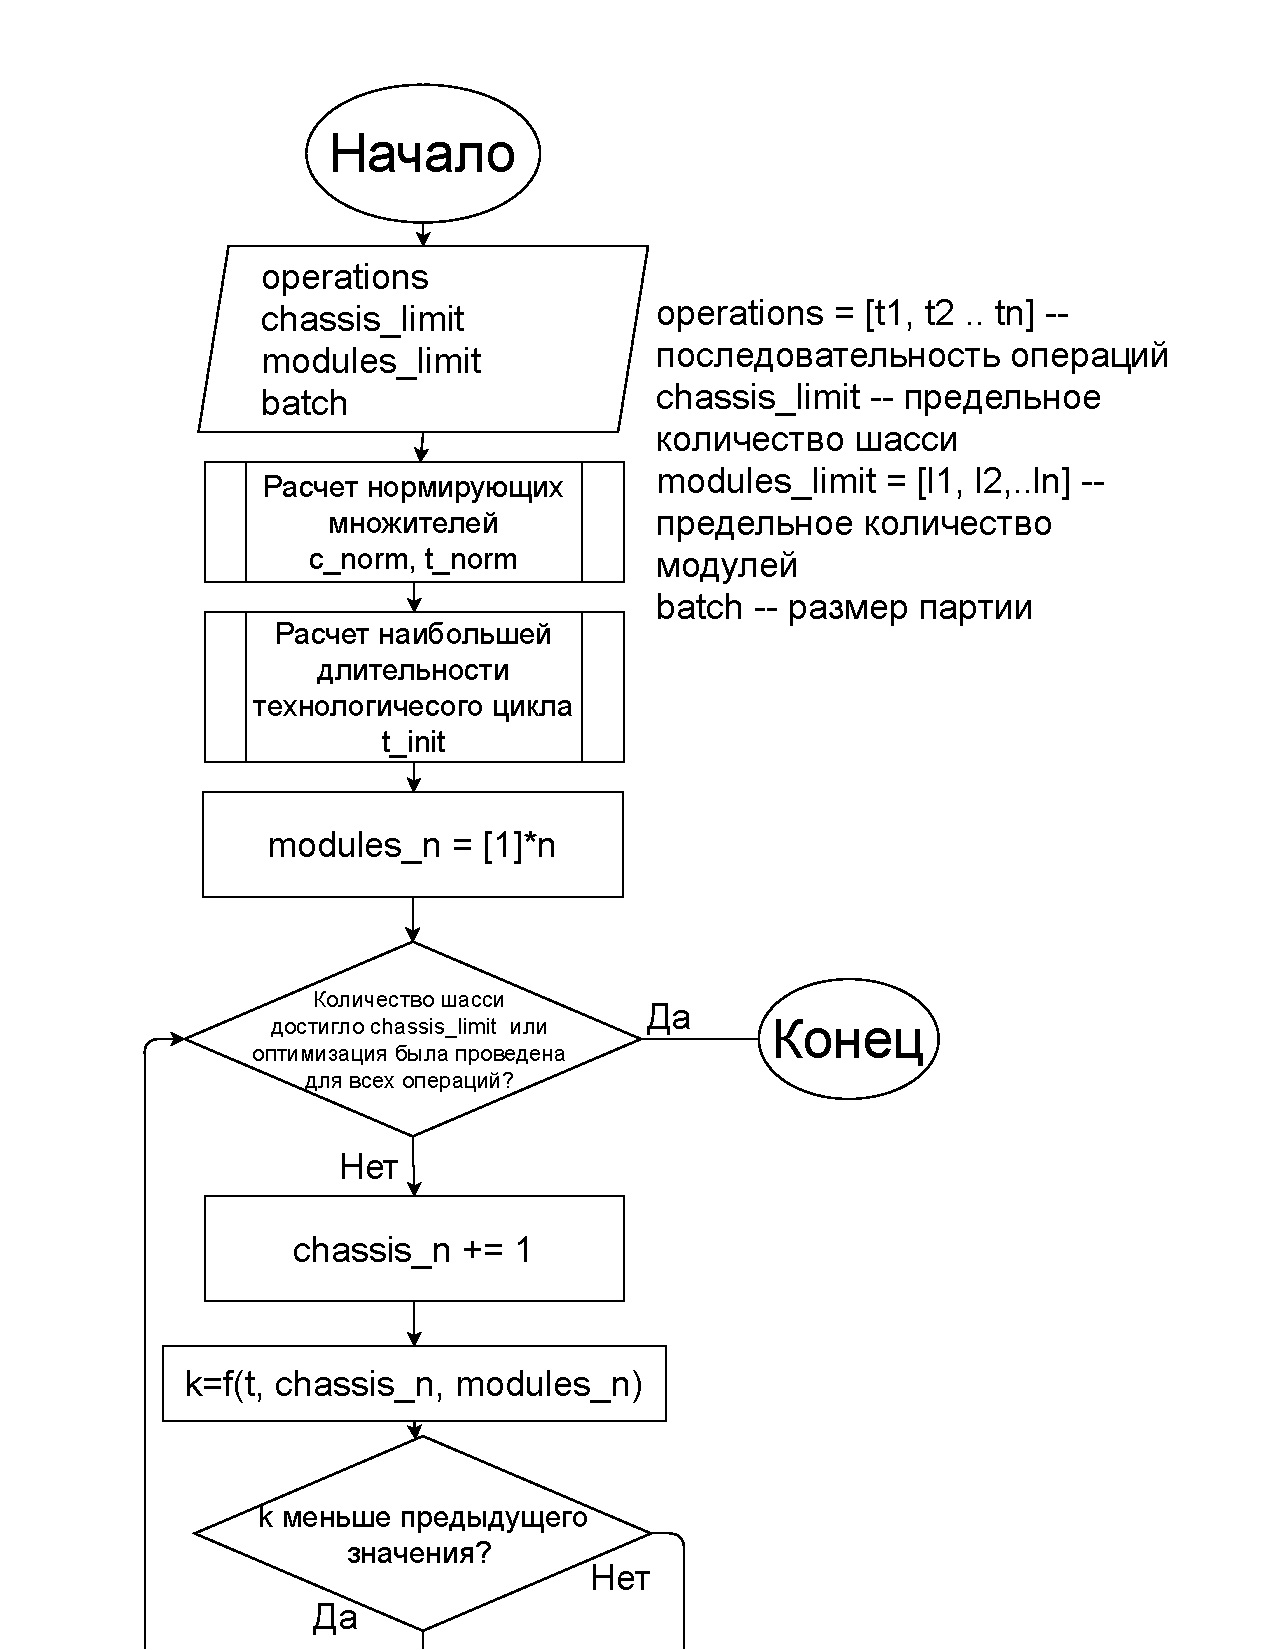
\includegraphics[width=0.6\textwidth]{ch-2/algo-1}
	}
	\caption{Блок схема алгоритма оптимизации (начало)}\label{fig:algo-1}
\end{figure}

\begin{figure}[!t]
	\centerfloat{
		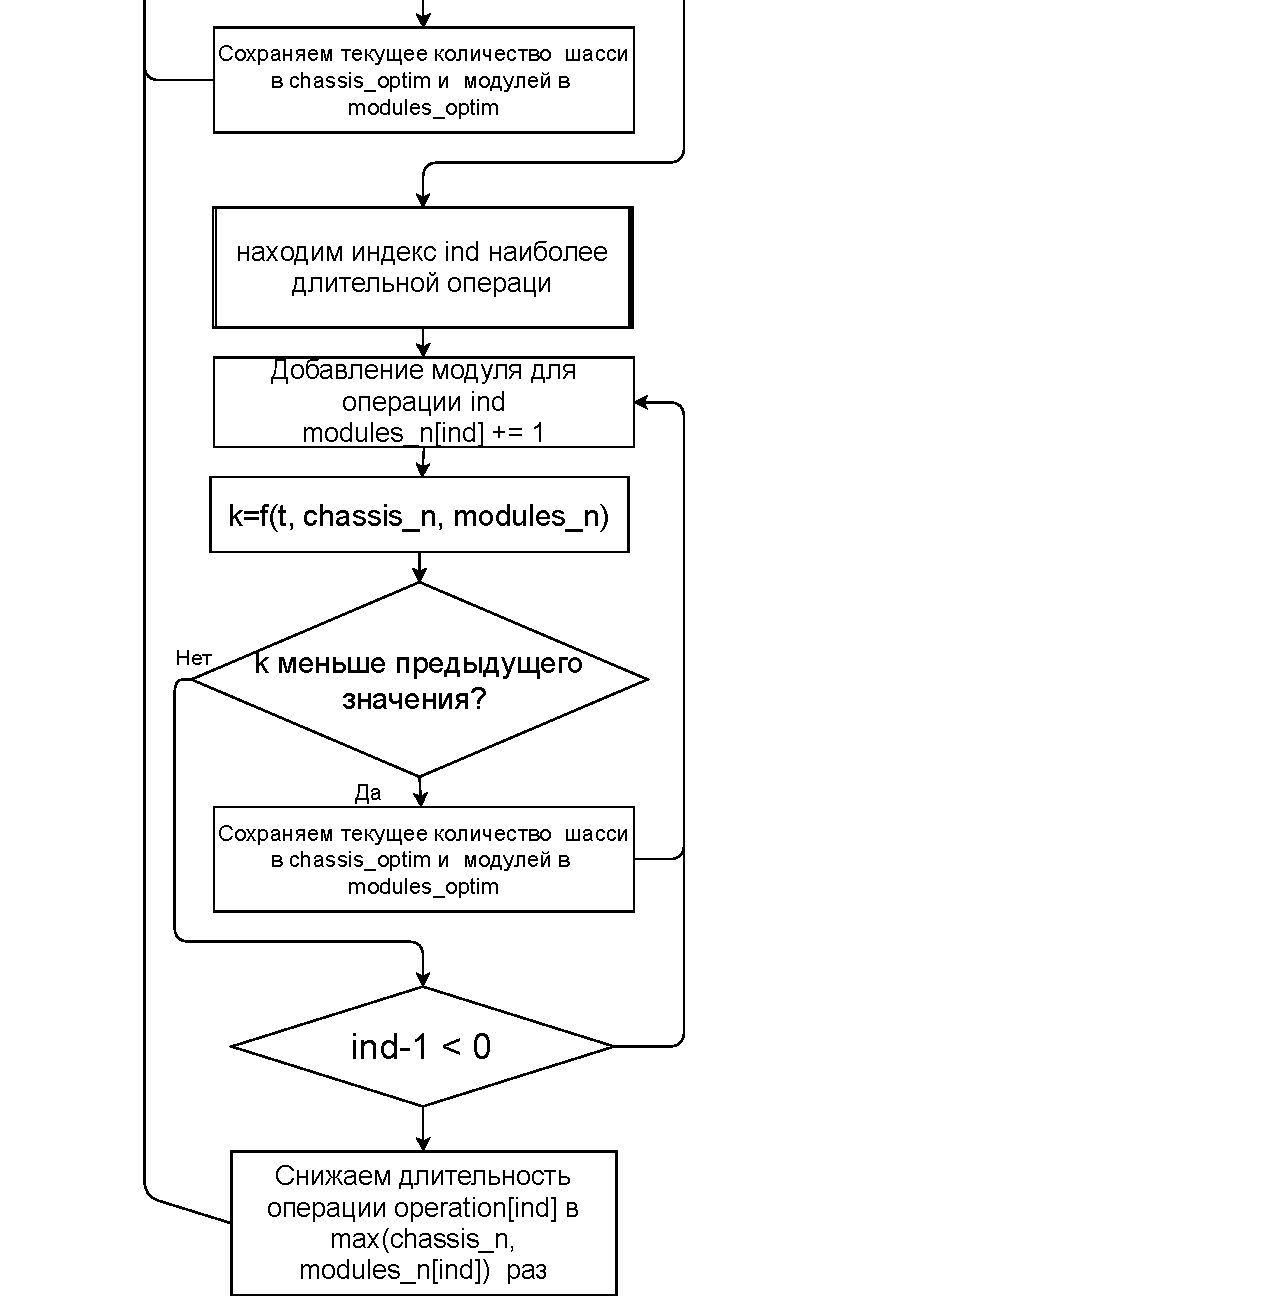
\includegraphics[width=0.6\textwidth]{ch-2/algo-2}
	}
	\caption{Блок схема алгоритма оптимизации (окончание)}\label{fig:algo-2}
\end{figure}


\paragraph{Первый этап.} На первом этапе производится расчёт нормирующих множителей. Значение нормирующего множителя \texttt{c\_norm} приравнивается  количеству видов модулей. То есть, если имеется 5 разных классов операций, выполняемых на модульном оборудовании, \texttt{то c\_norm = 5}. Затем необходимо определить нормирующий множитель технологического цикла \texttt{t\_norm}. Для этого производится расчёт длительности процесса для случая, когда \texttt{chassis\_n = c\_norm}, а \texttt{modules\_n} является единичным списком \texttt{[1, 1, 1...]}, длина которого совпадает с количеством классов модулей.  
 
\paragraph{Второй этап.} На этом этапе производится расчёт наихудшего варианта длительности \texttt{t\_init}.
Наихудший вариант может быть получен, когда имеется только одно шасси \texttt{chassis\_n = 1} и по одной единице модулей каждого вида \texttt{modules\_n = [1,1,1 ...]}. После чего для наихудшего варианта рассчитывается целевая функция \texttt{k\_prev = f(t, chassis\_n, modules\_n)}.

\paragraph{Третий этап.} Этот и дальнейшие шаги происходят в цикле. Цикл длится пока не будет превышен предел количества шасси или не будет проведен расчёт для каждой операции.

\begin{enumerate}
	\item Операции сортируются в порядки убывания длительности. При этом формируется список индексов операций. Затем значение индекса наиболее длительной операции сохраняется. Например, для \texttt{operations = [347.2, 1384.2, 437.7]} список индексов будет \texttt{indices[1, 2, 0]} и индекс наиболее длительной операции \texttt{ind = 1}.
	\item На этом шаге количество шасси инкрементируется  \texttt{chassis\_n += 1}. Рассчитывается длительность технологического  цикла \texttt{t}, после чего определяется значение  целевой функции \texttt{f(t, chassis\_n, modules\_n)}.
	\item Если результат целевой функции строго меньше предыдущего значения, то  текущее значение целевой функции сохраняется. Также сохраняются значения количества шасси и модулей, поскольку являются  оптимальными на данный момент. Переход обратно на шаг 1. В противном случае переход к шагу 4.
	\item Инкрементируется количество модулей, необходимых для операции с индексом \texttt{ind}. Это сопровождается расчётом целевой функции на каждой итерации. 
	\item Если значение целевой функции строго меньше предыдущего, то значения количества шасси и модулей сохраняются как оптимальное значение на данный момент, после чего переход к шагу 4. В противном случае происходит декремент индекса операции \mbox{\texttt{ind -= 1}} (предшествующая операция) и переход на шаг~4. Однако если операция первая, т.\,е. \texttt{ind - 1 < 0}, то сокращаем длительность операции в \texttt{min(chassis\_n, modules\_m[ind])} раз и переходим к шагу~1.
\end{enumerate}

Асимптотическая сложность для худшего случая полученного алгоритма $\mathcal{O}(n \cdot 2)$, против экспоненциальной сложности прямого перебора $\mathcal{O}(l^n)$, где $l$ "--- предельное количество модулей и шасси.
Для лучшего случая асимптотическая сложность будет $\mathcal{O}(n)$, в то время как прямой перебор все равно потребует проверки всех значений, т.\,е. его сложность будет $\mathcal{O}(l^n)$.


\subsection{Длительность технологического цикла}

Технологический цикл является частью производственного цикла, который представляет собой период от запуска детали (или партии деталей) в производство до получения готовой детали (или партии деталей). Длительность производственного цикла состоит из трех периодов:

\begin{itemize}
	\item Рабочее время.
	\item Технологический цикл.
	\item Время вспомогательных операций.
	\item Время естественных процессов, которые протекают без оказания воздействия на предмет труда человеком или оборудованием, но при этом происходит изменение состояния изделия.
	\item Время перерывов в работе, к ним относятся регламентированные и нерегламентированные перерывы. К нерегламентированным относятся перерывы обусловленные организационными и техническими причинами, например отказы оборудования.
\end{itemize}

Технологический цикл представляет собой период времени выполнения  всех основных технологических операций изготовления детали или суммой однооперационных циклов. Где однооперационный цикл "--- это время выполнения одной операции над партией деталей. Длительность технологического цикла может оказывать значительное влияние на весь производственный цикл в целом.~\footnote{Электронный ресурс: {\tiny\url{http://de.ifmo.ru/bk_netra/page.php?tutindex=3&index=107}} (дата обращения 12.12.2018).} Таким образом управление длительностью технологического цикла позволяют влиять на такие важные факторы производства как:

\begin{itemize}
	\item Производительность труда.
	\item Объёмы выпуска.
	\item Себестоимость окончательного изделия.
	\item Наличие незавершенного производства.
\end{itemize}

Перемещение предметов труда по технологическому циклу может происходит тремя способами:

\begin{itemize}
 	\item Последовательным.
	\item Параллельным.
    \item Последовательно-параллельным.
\end{itemize}

Последовательный цикл~(рисунок~\cref{fig:seq}) чаще всего используется на мелкосерийном и единичном производстве и представляет собой движение всей партии детали целиком -- от одной операции к другой. Переход на другую операцию осуществляется только в тот момент, когда на предыдущей обработаны все детали партии.
Его время вычисляется по формуле~\cref{eq:sc}:

\begin{figure}[!htb]
	\centerfloat{
		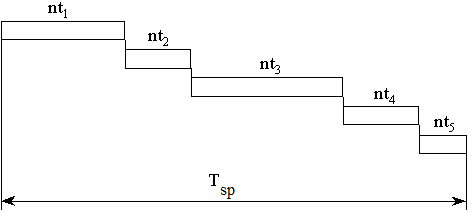
\includegraphics[width=0.5\textwidth]{ch-2/seq}
	}
	\caption{График последовательного вида движения}\label{fig:seq}
\end{figure}

\begin{equation}
T_{sc} = n t_{1} + n t_{2} + \ldots + n t_{K_0} = n \sum_{j=1}^{K_{0}}t_{j},
\label{eq:sc}
\end{equation}


\noindent где: $n$ "--- количество изделий в партии, $K_{0}$ "--- число операций обработки в соответствии с технологическим процессом,  $t_{j}$ "--- штучно-калькуляционное (операционное) время на $j$-ю операцию.

В отличии от последовательного движения при параллельное движении~(рисунок~\cref{fig:parallel}) передача детали от операции к операции происходит поштучно или транспортными партиями, на которые разбивается основная. Зачастую используется в серийном и массовом производстве, однако возможно применение и в мелкосерийном.

Длительность в таком случае рассчитывается по формуле~\cref{eq:pc}:

\begin{figure}[!htb]
	\centerfloat{
		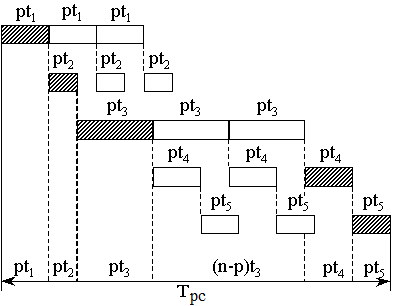
\includegraphics[width=0.5\textwidth]{ch-2/parallel}
	}
	\caption{График параллельного вида движения}\label{fig:parallel}
\end{figure}

\begin{equation}
T+{pc} = p\sum_{j=1}^{K_{0}}t_{j}+(n-p)t_{main},
\label{eq:pc}
\end{equation}

\noindent где: $p$ "--- размер транспортной партии, кратный целой партии $n$.

Параллельно-последовательный вид движения~(рисунок~\cref{fig:seq-parallel}) представляет собой сочетание двух предыдущих походов~\cref{eq:spc}. Передача детали осуществляется поштучно или транспортными партиями. При этом начало обработки на следующей операции происходит со смещением, таким образом, чтобы избавиться от микропауз, возникающих в последовательном типе движения . Однако применяется по большей части только при массовом и крупносерийном производстве, поскольку требует налаженного ритма производства.

\begin{figure}[!htb]
	\centerfloat{
		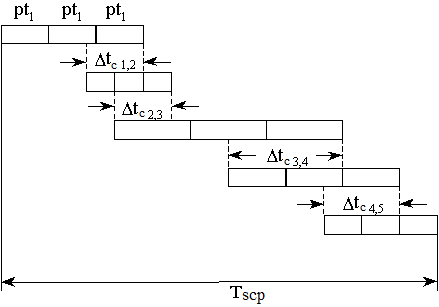
\includegraphics[width=0.5\textwidth]{ch-2/seq-parallel}
	}
	\caption{График параллельно-последовательного вида движения}\label{fig:seq-parallel}
\end{figure}

\begin{equation}
T_{spc} = T_{sc} - \sum_{j=1}^{K_{0}-1}\Delta t_{c \;  j,j+1} = n \sum_{j=1}^{K_0}t_j-(n-p)\sum_{j=1}^{K_{0}-1}t_{short \; j,j+1},
\label{eq:spc}
\end{equation}

\noindent где: $Delta t$ "--- разность времени пары смежных операций, $t_{short}$ "--- время кратчайшей из пары смежных операций. 

Для расчета критерия оптимизации на каждой итерации требуется определение длительности технологического цикла. Вместе с этим применение концепции модульного оборудование позволяет не просто применять последовательный вид движения, но и использовать транспортные партии попеременного размера. Это обуславливается тем фактом, что часть технологического оборудования можно реконфигурировать в процессе технологического цикла повышая или понижая производительность того или иного однооперационного цикла.  Это в свою очередь позволяет уменьшить длительность технологического цикла в сравнении с немодульным оборудованием.

%-----------------------------------------------------------------------------------------------------------------------------------------------

%\section{Математическая модель унификации, параметризации и оптимизации компонентов модульной технологической платформы}
%
%\section{Модель оптимизации модульного оборудования при единичном и мелкосерийном производствах}

%Рассмотрим основные понятия оптимизации по номенклатуре выпускаемых изделий. Пусть $N$ "--- номенклатура групп изделий, предлагаемая для выпуска, полученная на этапе маркетинговых исследований:



%\noindent где $D_i$ "--- группа изделий. Группирование происходит по технологическому признаку [Митрофанов, стр. 43] "--- \textit{вид обработки}.
%
%
%
%\noindent где $P_j$ "--- групповая технологическая операция. В соответствие каждой группе ставится вероятность спроса:
%
%\begin{equation}
%f: D_i \rightarrow \upsilon_i, D_i \in N, \upsilon_i \in V,
%\end{equation}
%
%\noindent где $V$ "--- множество вероятностей такое, что:
%
%\begin{equation}
%\forall\upsilon\in V: \upsilon\leq 1 \wedge\upsilon > 0
%\end{equation}
%
%Определим композицию для нахождения наиболее вероятной группы или нескольких групп:
%
%\begin{equation}
%g: V \rightarrow N', \forall\upsilon = V_max: \upsilon \in f(N'), V_max \in V, N' \subset N
%f \ g = h,
%\end{equation}
%
%\noindent где $N' = (D_j)_{j \in J}$ "--- результат композиции (семейство наиболее вероятных групп), $\bigcup N' = {p:p_1\in D_1 \vee p_2\in D_2 \vee\ldots\vee p_j\in D_j}$ "--- множество групповых операций в этих группах.
%
%Фактическая номенклатура задаётся нечётким множеством:
%
%\begin{equation}
%N'' = {(D, \upsilon(D)) \mid D \in N}
%\end{equation}
%
%Определить коэффициенты целесообразности использования модульности можно как:
%
%\begin{equation}
%\epsilon = \frac{\big|\bigcup N' \big|}{|G|},
%\end{equation}
%
%\noindent где $G$ "--- домен операций, $\bigcup\limits_{i} N$. Если $\epsilon\rightarrow 0$ "--- модульность целесообразна, если $\epsilon\rightarrow 1$ "--- модульность нецелесообразна.

%\section{Определение критерия оптимизации конфигурации модульного оборудования}
%
%\section{Разработка параметрического ряда ширины присоединительной поверхности}

\section{Выводы по главе 2}

В настоящей главе было проведено исследование методик проектирования и применения модульного оборудования. Были рассмотрены подходы к унификации оборудования, а также существующие стандарты унификации. На основании проведённого анализа можно сделать вывод о том, что на сегодняшний день не существует единого подхода к унификации и стандартизации модульного оборудования, однако отдельные методики унификации описаны и стандартизированы. Именно на их основании можно проводить унификацию модульного оборудования. 

Далее рассматриваются особенности проектирования модулей. Отмечается, что на модули в первую очередь должны быть наложены ограничения, связанные с удобным и быстрым креплением модулей. Поэтому основное внимание нужно уделить конструкции сопрягаемых поверхностей и способу крепления. На основании сформулированных требований к устройству крепления модулей предлагается система быстрой установки модулей, основанная на применении специальной формы сопрягаемых поверхностей с направляющим пазом и элекромагнитом.

На основании предложенной конструкции системы крепления выбирается ряд параметров модуля, из которых выбирается главный параметр, также задаются фиксированные параметры. Главным параметром выбрана грузоподъемность электромагнита. В качестве основных параметров выбраны: ширина присоединительной поверхности модуля, глубина модуля, ширина модуля, ток потребления модуля. В качестве фиксированных параметров приняты напряжение питания, геметрические параметры ответной части паза крепления. Для модулей с электромагнитным креплением было выявлено пять ограничений: ограничение массы модуля в зависимости от грузоподъемности электромагнита, ограничение грузоподъемности электромагнита в зависимости грузоподъемности шасси, ограничение тока потребления модуля в зависимости от максимального рабочего тока шасси, ограничение глубины модуля в зависимости от размера рабочего пространства, ограничение на ширину присоединительной поверхности модуля. На основании параметров и ограничений предложены основные кратные ряды для модулей.

Следующим пунктом предложена методика расчёта показателя целесообразности применения модульного оборудования. За основу показателя целесообразности взята метрика общей эффективности оборудования, модифицированная для случай применения модульного оборудования в мелкосерийном и единичном производстве. Показатель целесообразности позволяет оценить перспективы использования модульного оборудования для типовых технологических процессов, используемых на предприятии. Для проверки правильности данного критерия, был разработан технологический процесс изготовления изделия <<гироподвес>>, после чего проведен расчёт критерия целесообразности, который показал, что для данного технологического процесса с заданным годовым объёмом выпуска. Результат расчёта показал, что применение предложенного критерия целесообразно. Далее, для проверки правильности данной гипотезы, была проведен ряд вычислительных экспериментов в среде дискретно-событийного моделирования AnyLogic, который показал, что при использовании модульного оборудования для данного технологического процесса прирост производительности составляет~\SI{18}{\percent} из чего можно сделать вывод о том, что математическое описание критерия целесообразности было определено верно.

Следующим этапом исследования вопросов повышения эффективности применения модульного оборудования стала разработка методики оптимизации комплекта модульного оборудования, то есть определения наиболее оптимального состава модулей и шасси для конкретного технологического процесса. Первоначально был определён критерий оптимизации. Для парка модульного технологического оборудования было выделено два критерия "--- стоимость предлагаемого комплекта оборудования и длительность технологического цикла. С помощью метода аддитивной свертки был произведён переход от двухкритериальной оптимизации к однокритериальной. Была описана целевая функция нормирования признаком, а произведён расчёт весовых коэффициентов. Суть алгоритма оптимизации заключается в итерации от главной операции (зачастую являются узким местом)  к менее главным, сопровождающейся добавлением шасси и модулей, а затем оценкой значения целевой функции. Главной операцией считается операция с наибольшей длительностью. 

\FloatBarrier